\documentclass{beamer}
\usepackage[utf8]{}
\usepackage{hyperref}
\usepackage[T1]{fontenc}
\usepackage{tikz}
\usepackage{listings}
\usepackage{algorithm,algorithmic}
\usepackage{amsmath}
\usepackage{pifont}
\usepackage{color}
\usepackage{svg}
\svgpath{{./images/}}
\usepackage{colortbl}
\usepackage[
    type={CC},
    modifier={by-nc},
    version={4.0},
    imageposition = right
]{doclicense}
\usepackage{ragged2e}
\usepackage{Wue}

\colorlet{shadecolor}{gray!40}

\usepackage{wrapfig}

\setbeamertemplate{itemize items}[square] 
\usepackage[backend=biber,style=numeric-comp,sorting=none]{biblatex}


\author{Di Battista Mattia}
\title{Distributed Systems and Cloud Computing: Election Distributed Algorithms}

\institute{Università degli Studi di Roma "Tor Vergata"} 

\usefonttheme[onlymath]{serif}

\begin{document}

\defverbatim[colored]\lstI{
\begin{lstlisting}[language=Python,basicstyle=\footnotesize\ttfamily,keywordstyle=\color{blue}]
def set_logging() -> logging:
    logging.basicConfig(level=logging.DEBUG,
        format="[%(levelname)s]%(asctime)s\n%(message)s",
        datefmt='%b-%d-%y %I:%M:%S'
    )
return logging
\end{lstlisting}
}

\defverbatim[colored]\lstII{
\begin{lstlisting}[language=Python,keywordstyle=\color{blue},basicstyle=\footnotesize\ttfamily,xleftmargin=.1\textwidth]
def delay(flag: bool, ub: int):
    if flag:
        delay = randint(0, floor(ub*1.5))
        time.sleep(delay)
\end{lstlisting}
}

\defverbatim[colored]\lstIII{
\begin{lstlisting}[language=Python,basicstyle=\footnotesize\ttfamily,keywordstyle=\color{blue},xleftmargin=.3\textwidth,xrightmargin=.70\textwidth]
class Type(Enum):
    ELECTION = 0
    END = 1
    ANSWER = 2
    HEARTBEAT = 3
    REGISTER = 4
    ACK = 5
\end{lstlisting}
}

\defverbatim[colored]\lstIV{
\begin{lstlisting}[language=Python,basicstyle=\footnotesize\ttfamily,keywordstyle=\color{blue},xleftmargin=.1\textwidth,xrightmargin=.75\textwidth]
def __init__(self, ...):
    ...
    self.lock = Lock()
    thread = Thread(target=self.listening)
    thread.daemon = True
    thread.start()
    self.start_election()
    Algorithm.heartbeat(self)
\end{lstlisting}
}

\defverbatim[colored]\lstV{
\begin{lstlisting}[language=Python,basicstyle=\footnotesize\ttfamily,keywordstyle=\color{blue},xleftmargin=.1\textwidth]
self.lock.acquire()
if self.participant or (self.coordinator in
    [self.id, DEFAULT_ID]):
    self.lock.release()
    continue
\end{lstlisting}
}

\defverbatim[colored]\lstVI{
\begin{lstlisting}[language=Python,basicstyle=\footnotesize\ttfamily,keywordstyle=\color{blue}]
def kill_node(self, port: int):
    for proc in process_iter():
        for conns in proc.connections(kind='inet'):
            if conns.laddr.port == port:
                proc.send_signal(signal.SIGINT)
\end{lstlisting}
}

	\begin{frame}
    \titlepage
    \centering
    \doclicenseIcon
    \end{frame}

	
	\begin{frame}{Outline}
		\tableofcontents
	\end{frame}
	
	\section{Goal}
		    \begin{frame}{Goal}
		    
		    The aim is to implement: 
		    
		    \begin{itemize}
		        \item \textbf{Chang and Roberts} algorithm
		        \item \textbf{Bully} algorithm
		        \item Several services (i.e., register, heartbeat, verbose, delay)
		        \item Test suite
		    \end{itemize}\pause
		    Deployment on \textbf{AWS EC2} instance using \textbf{Docker} containers
		    \end{frame}
		    
	\section{Service}
	    
	    \subsection{Register Service}
	    
    	    \begin{frame}{Register Service (1)}
            
            \textbf{Register service} aims to:
            
            \begin{itemize}
                \item provide knowledge of the entire network to all nodes belonging to it
                \item generate a unique random ID for each member of the topology
            \end{itemize}\pause
            
            Settings are:
            \begin{itemize}
                \item \textbf{TCP} port where the register node is listening
                \item listening window is kept open for a \textit{SOCKET\_TIMEOUT}
            \end{itemize}\pause
            
            
            Two sockets are created:
            \begin{enumerate}
                \item to communicate with the register node
                \item to listen to eventual packets from other nodes
            \end{enumerate}
    	    \end{frame}
	        
	        \begin{frame} {Register Service (2)}
	           
	       E.g., of the \textbf{register phase} from three generic nodes and register node:
	        \begin{center}
	         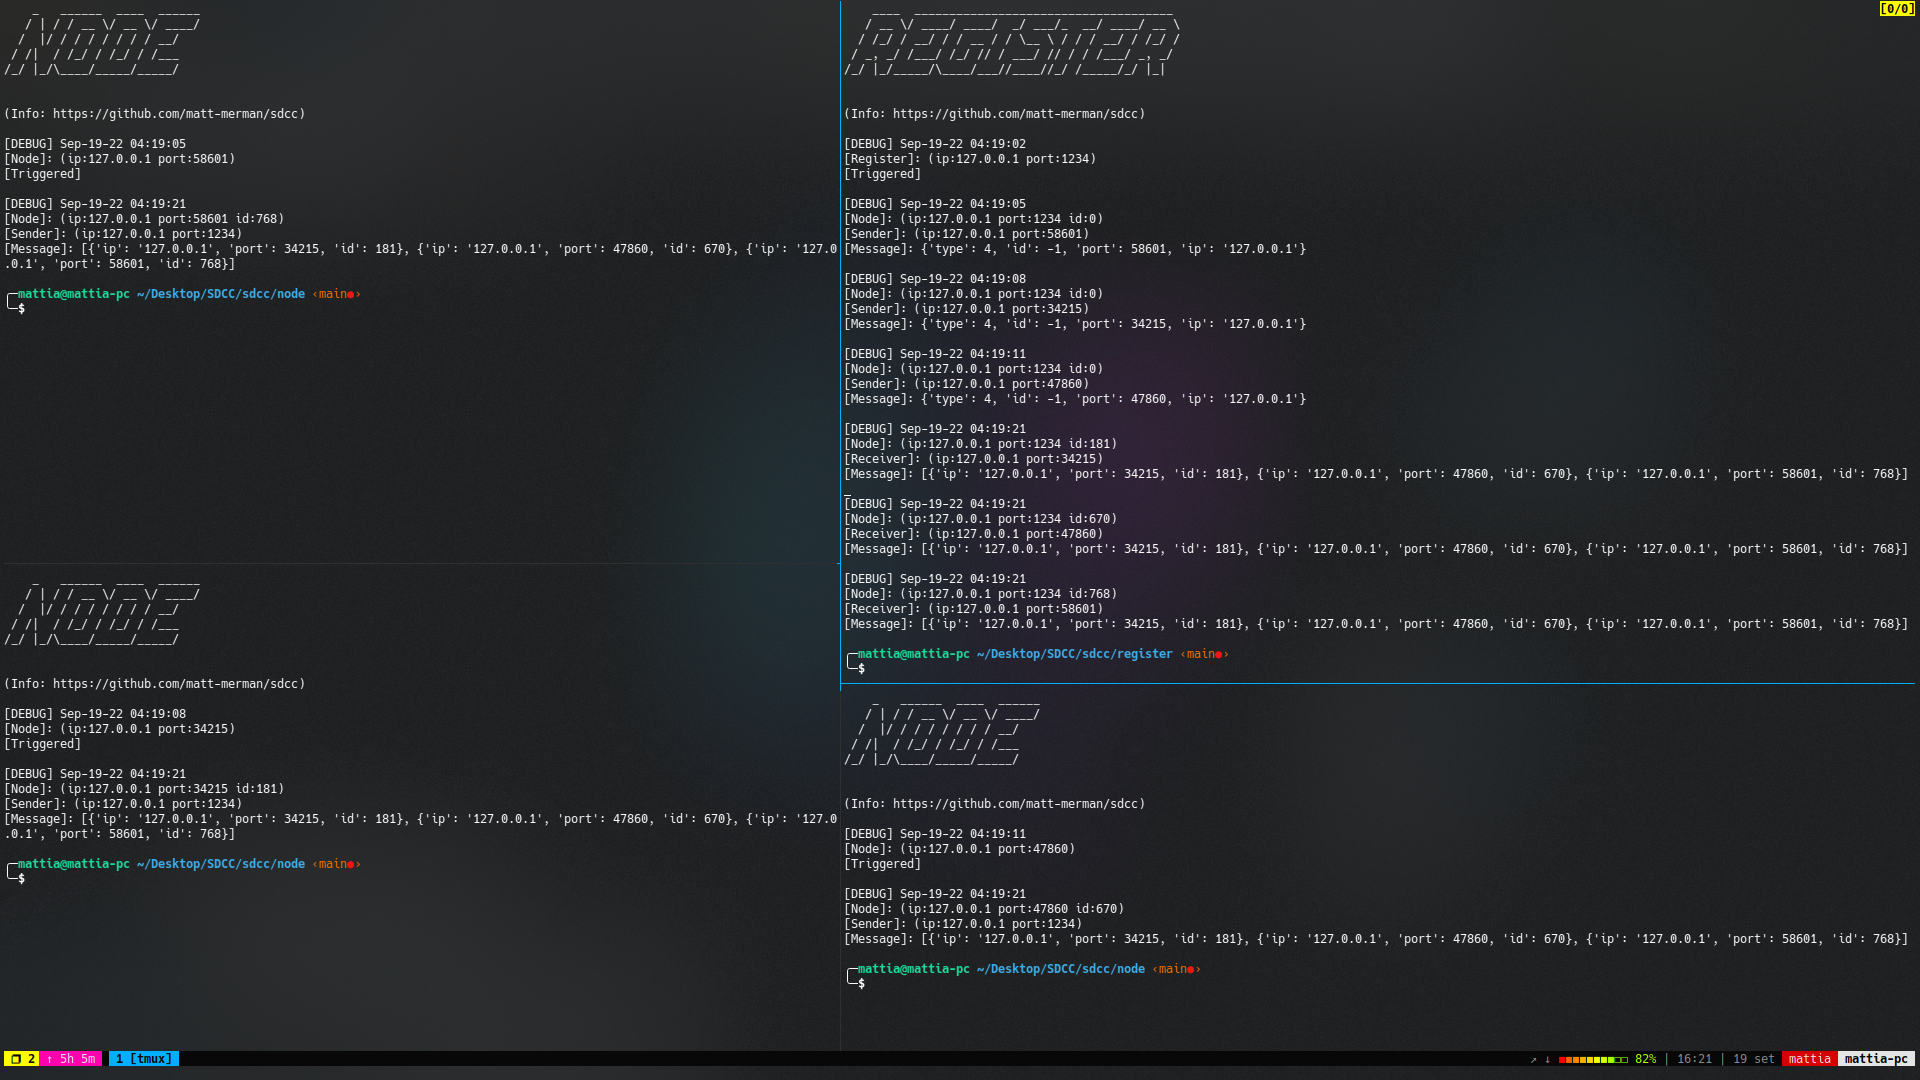
\includegraphics[width=.8\textwidth]{images/register_terminal.png}
	     \end{center}
	        
	        \end{frame}
	        
	    \subsection{Heartbeat Service}
	    
	    \begin{frame}{Heartbeat Service}
	    
	   \begin{columns}
	    \column{.5\textwidth}
	    
	    \textbf{Heartbeat service} allows detaching crashes by the coordinator node
	    
	    \begin{itemize}
	        \item a thread heartbeats the leader through a dedicated \textbf{TCP} socket
	    \end{itemize}
	    \pause
	    
	    Settings are:
	    
	    \begin{enumerate}
	        \item period waited to receive the ACK message
	        \item period waited to send the HEARTBEAT message
	    \end{enumerate}
	    
	    \column{.5\textwidth}
	    
	    \begin{figure}
          \centering
          \includesvg[inkscapelatex=false, width=1.1\textwidth]{heartbeat.svg}
          \caption{Heartbeat service invoked by two nodes}
        \end{figure}
	     \end{columns}
	     
	    \end{frame}
	    
	    \subsection{Verbose Service}
	    
	    \begin{frame}{Verbose Service}
	    
	    \textbf{Verbose service} shows all messages exchanged (i.e., received, sent) throughout the node lifetime. Main info shown are:
        \begin{itemize}
            \item timestamp
            \item node info (i.e., IP address, port number, ID)
            \item receiver/sender info (i.e., IP address, port number, ID)
            \item message content
        \end{itemize}	
        
        \pause
        
        \textbf{Logging} library is used to define the message syntax
        
        \lstI
        
	    \end{frame}
	    
        \subsection{Delay Service}
        
        \begin{frame}{Delay Service}
        \textbf{Delay service} generates a period waited by the sender to forward the current packet
        \begin{itemize}
            \item causing the receiver timeout to expire
        \end{itemize}
        \lstII
        \begin{itemize}
            \item activated by default when tests are performed
        \end{itemize}
	    \end{frame}
	    
	 \section{Algorithm}
	 
	 \subsection{Implementation}
	 
	 \begin{frame}{Implementation (1)}
	 
	 \begin{columns}
	 
	 \column{.35\textwidth}
	 \textbf{Implementation} consists of:
	 \begin{itemize}
	     \item abstract class
	     \item election distributed algorithms classes
	     \begin{itemize}
	         \item[\ding{113}] as child class to extend the first one
	     \end{itemize}
	 \end{itemize}
	 
	 \column{.65\textwidth}
    \begin{figure}
          \centering
          \includesvg[inkscapelatex=false, width=\textwidth]{class.svg}
          \caption{Logic implementation of the classes}
        \end{figure}
	     
	 \end{columns}
	     
	 \end{frame}
	 
	 \begin{frame}{Implementation (2)}
	 	 
	 	 Six \textbf{types of messages} can be exchanged between nodes:
	 	 
	 	 \lstIII
	 	 
	 	 \begin{itemize}
	 	     \item ANSWER type is used by the \textbf{Bully algorithm} 
	 	     \item REGISTER type is sent during register phase
	 	 \end{itemize}
	 	 
	 	 \end{frame}
	 	
	 \begin{frame}{Implementation (3)}
	 
	 Algorithms begin with run the \textbf{listening thread} after which they start an election
	 \begin{itemize}
	     \item after completing these two phases the heartbeat can start
	 \end{itemize}
    
    \lstIV
	     
	 \end{frame}
	 
	 \begin{frame}{Implementation (4)}
	     \textbf{Lock} is defined to manage shared resources
	     \begin{itemize}
	         \item many data are accessed simultaneously from multiple threads 
	     \end{itemize}
	     
	     \begin{center}
	     \lstV
	     \end{center}


	 \end{frame}
	 
	 \subsection{Chang and Roberts Algorithm}
	 
	 \begin{frame}{Chang and Roberts Algorithm (1)}
	  
	   ID's node is used to define the \textbf{ring} network 
	   \begin{itemize}
	       \item next node is the one with the greatest ID then current and the lowest among others
	   \end{itemize} 
	   
	   \begin{figure}
          \centering
          \includesvg[inkscapelatex=false, width=.6\textwidth]{ring_1.svg}
          \caption{Election started by node with \textit{id=23} in ring topology}
        \end{figure}
        \end{frame}
        
        \begin{frame}{Chang and Roberts Algorithm (2)}
            
        Leader is removed from the nodes list
        \begin{itemize}
            \item remaining nodes can not interact with it even if it is still active
        \begin{itemize}
            \item[\ding{113}] when a leader crash occurs
            \item[\ding{113}] node's timer associated with a heartbeat message elapses
        \end{itemize}
        
        \end{itemize}
        
	 \end{frame}
	   
	 \subsection{Bully Algorithm}
	 
	 \begin{frame}{Bully Algorithm (1)}
	 
	 \textbf{Bully algorithm} assumes that each process knows which processes have higher identifiers
	 \begin{itemize}
	     \item it can communicate with all such processes
	 \end{itemize}
	 
	 \begin{figure}
          \centering
          \includesvg[inkscapelatex=false, width=.6\textwidth]{bully_1.svg}
          \caption{Election started by node with id=23}
        \end{figure}
        \end{frame}
        
        \begin{frame}{Bully Algorithm (2)}
	 
	 Possible \textbf{scenarios}: 
	   
	   \begin{enumerate}
	       \item leader delays sending the ACK packet 
	       \begin{itemize}
	           \item other nodes start a new election that will produce the next coordinator also if the previous one is running
	       \end{itemize}
	       \item leader is stopped 
	       \begin{itemize}
	        \item a new election will start 
	        \item all messages sent to the sleeping node are queued
	        \item will receive those messages and begin the leader again
	       \end{itemize}
	   \end{enumerate}
	   
	 \end{frame}
	 
	 
	 \section{Test Suite}
	 
	 \begin{frame}{Test Suite (1)}
	     Following \textbf{tests} are performed:
	     \begin{enumerate}
	        \item generic node fails
	        \item coordinator fails
            \item both generic and coordinator nodes fail
	 \end{enumerate}\pause
	 
	 To interrupt a specific node \textbf{psutil} library is used
	 \begin{itemize}
	     \item to kill a process that is listening on a certain \textbf{TCP} port
	 \end{itemize}
	 
	 \lstVI

	 \end{frame}
	 
	 \begin{frame}{Test Suite (2)}
	 
	 \textbf{Test execution} is interactive 
	 \begin{itemize}
	     \item user chooses which test executes 
	       \begin{itemize}
	           \item[\ding{113}] sees logging information on the terminal
	           \item[\ding{113}] sets which algorithm has to be performed
	       \end{itemize}
	 \end{itemize}
	 
	 \begin{center}
	  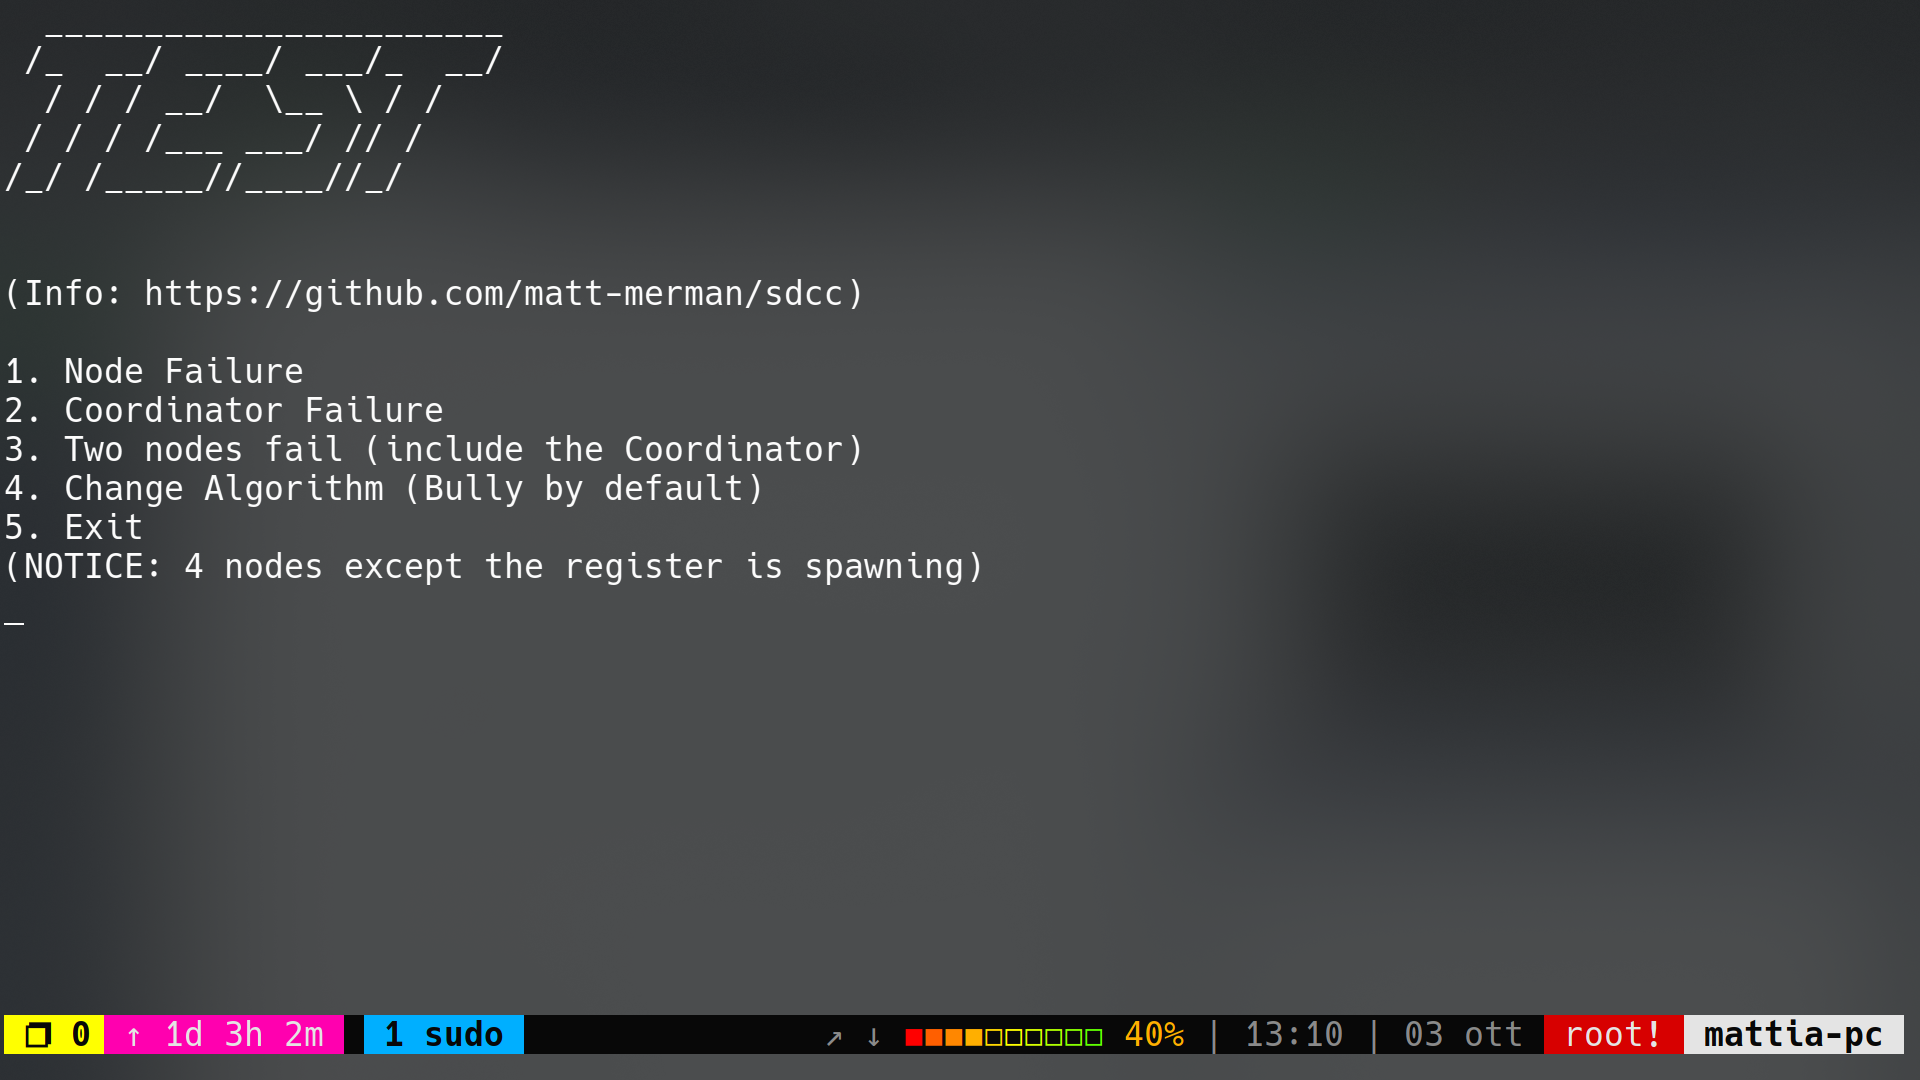
\includegraphics[width=.7\textwidth]{images/tests.png}
	 \end{center}
	 
	 	 
	 \end{frame}
	 
	 \section{Deployment}
	 
	 \begin{frame}{Deployment}
    	Network is deployed on an \textbf{AWS EC2} instance using  \textbf{Docker} container 
    	\begin{itemize}
    	    \item \textbf{Docker Compose} is used to automate the container’s creation
    	    \begin{itemize}
    	        \item[\ding{113}] creates a network where containers can communicate with each other
    	    \end{itemize}
    	    \item to automate the deployment procedure \textbf{Ansible} is used
    	    \begin{itemize}
    	        \item[\ding{113}] Docker installation
    	        \item[\ding{113}] to forward the code application on an EC2 instance
    	    \end{itemize}
    	\end{itemize}
    	\end{frame}
    	
    	\begin{frame}
    	
    	\begin{columns}
    	\column{.5\textwidth}
    	\begin{figure}
          \centering
          \includesvg[inkscapelatex=false, width=\textwidth]{arch.svg}
          \caption{Heartbeat service invoked by two nodes}
        \end{figure}
        
    	\column{.5\textwidth}
    	
    	 \begin{figure}
    	 \centering
	  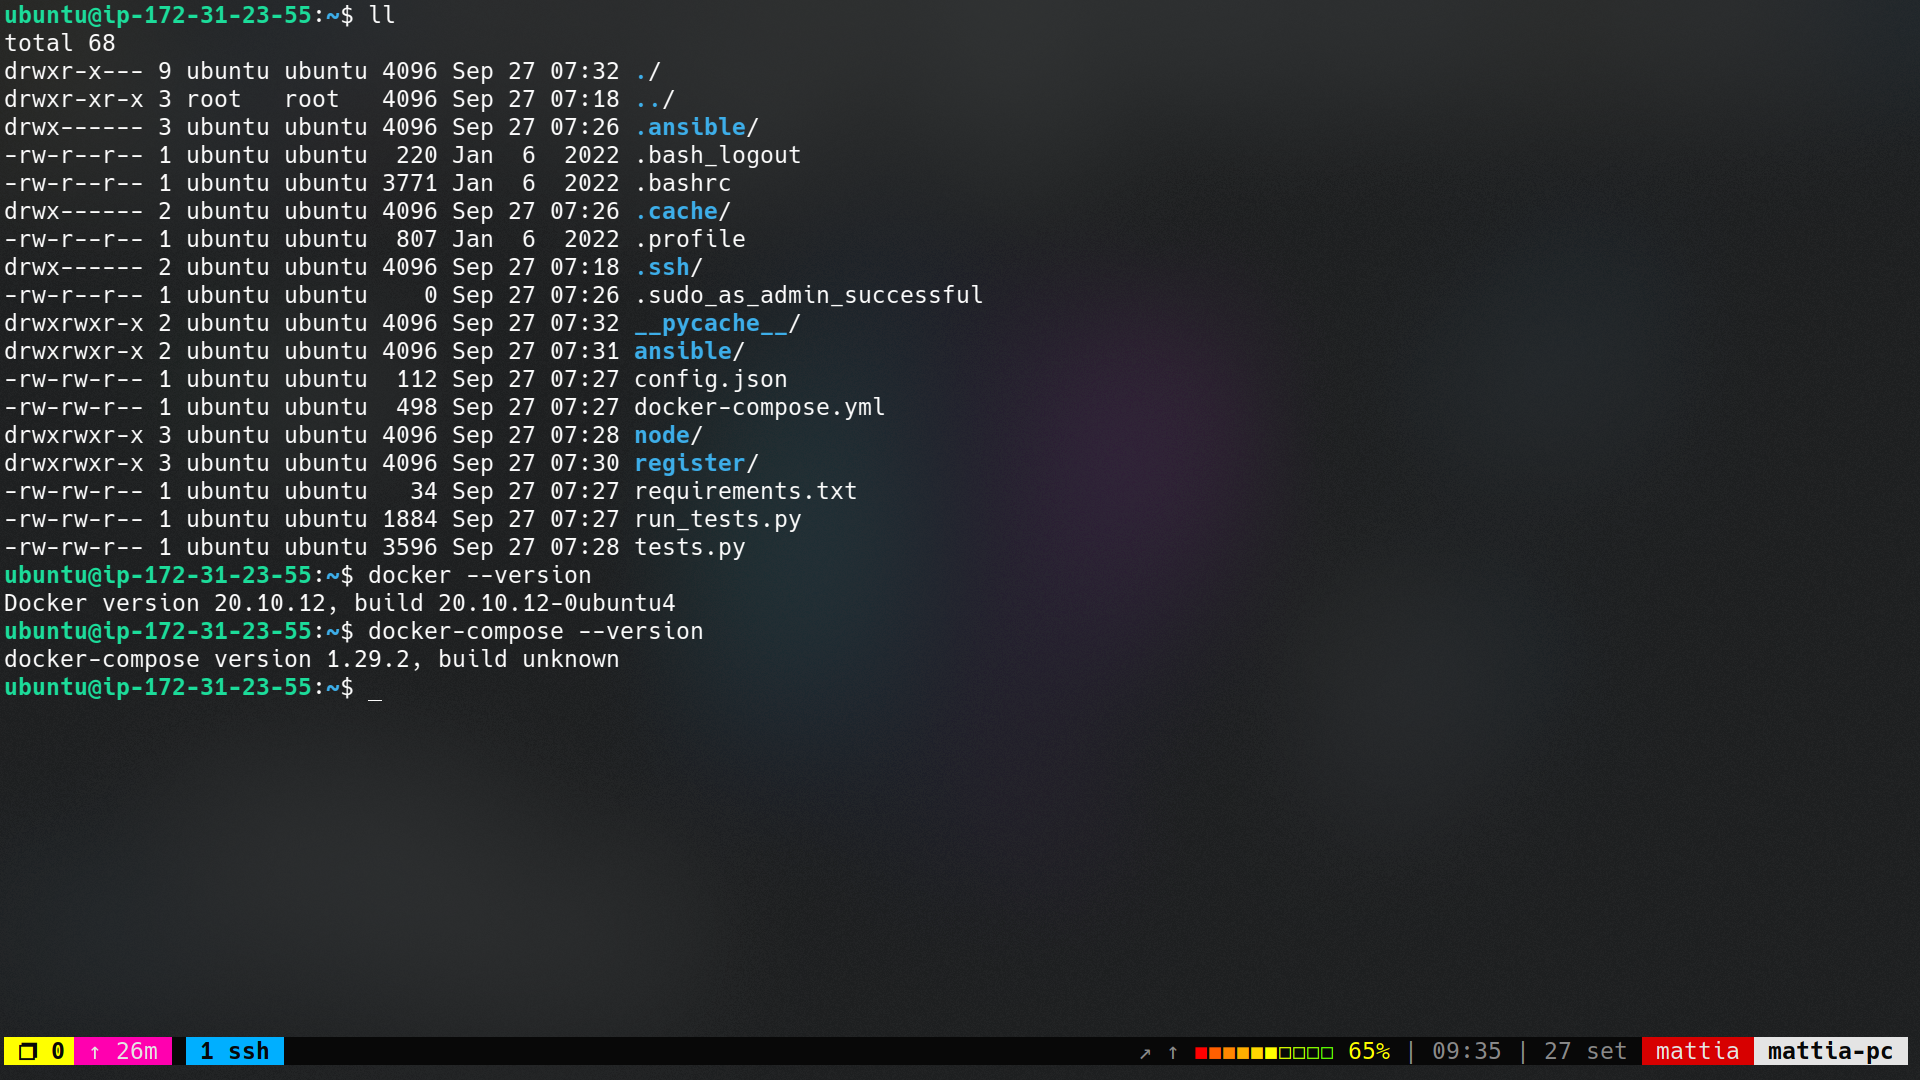
\includegraphics[width=\textwidth]{images/aws_demo.png}
	  \caption{Result from Ansible execution on an EC2 instance}
	 \end{figure}
    
    	
        \end{columns}
	 \end{frame}
	
\end{document}